%!TeX root = 5-diffusion.tex
\documentclass[main]{subfiles}

\begin{document}

\chapter{Xenon and krypton transport properties}
\vspace*{-1\baselineskip}


In separation processes, diffusion can either be the main performance metric or a neglected secondary parameter. There are actually two different use cases for separation using nanoporous materials: the adsorption-based separation that is mainly a thermodynamic process and the nanoporous separation membranes that relies on the kinetic properties. In a membrane-based process, the gas is sieved through a membrane material that blocks some molecules (e.g. Xe) and let other molecules (e.g.) diffuse freely. The performance of the separation is measured with the ratio of the diffusion coefficients instead of the thermodynamic selectivity we defined in chapter 2. The process of interest is, however, the adsorption-based separation performed industrially by pressure and/or temperature swing adsorption, and even if the thermodynamic selectivity is the main performance metric, the kinetic performances can improve our understanding of the adsorption process. For instance, in breakthrough experiments (a lab equivalent of a pressure swing adsorption) used to characterize the comparative adsorption performances of a gas mixture, the shape of the curve can be explained by diffusion processes. The goal of this chapter is to explore this often neglected diffusion parameter in an adsorption-based Xe/Kr separation process.

\begin{figure}[ht]
  \centering
    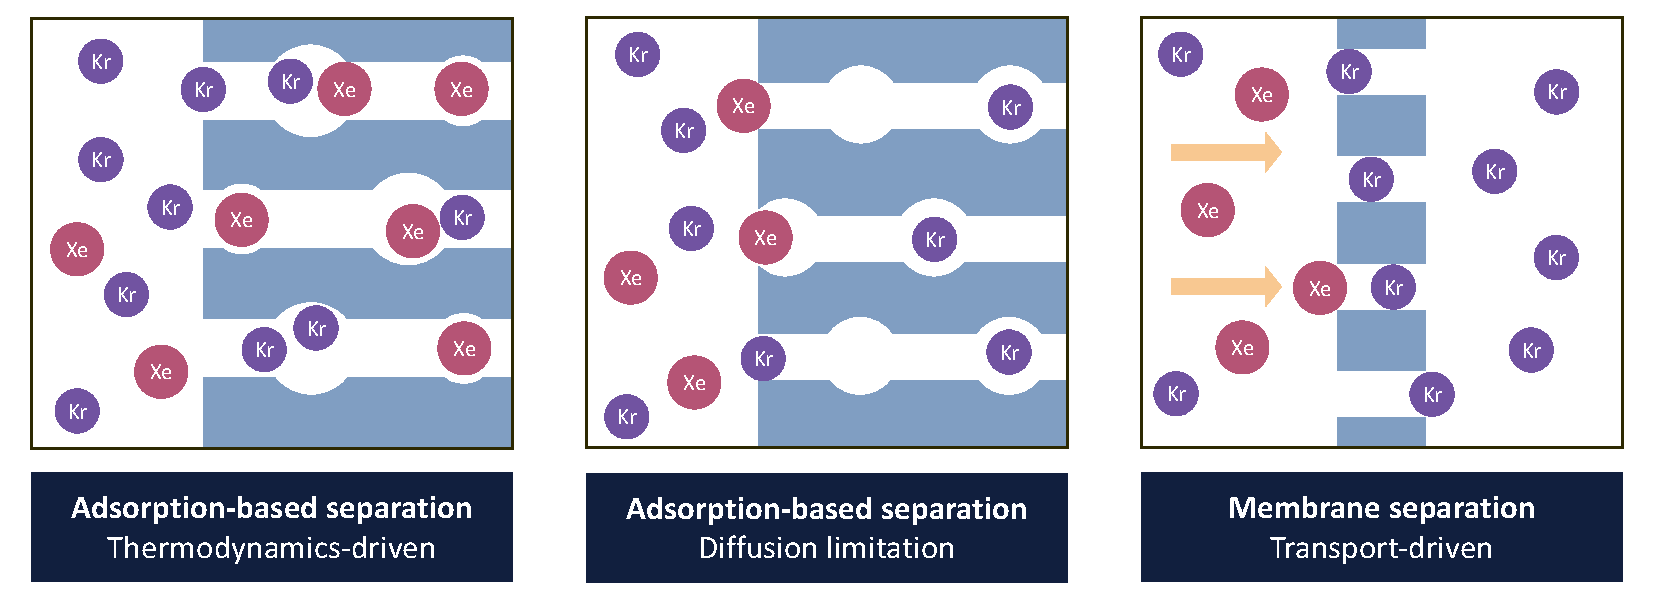
\includegraphics[width=0.95\textwidth]{figures/5-diffusion/Diffusion.pdf}
    \caption{Illustration of the comparative role of the thermodynamic and transport properties for Xe/Kr separation in nanoporous materials. From the transport dominated process of membrane separation to the thermodynamically equilibrated separation processes in the nanopores, different more nuanced cases could emerge where the diffusion imposes kinetic limitations. }
    \label{fgr:intro_diffusion}
\end{figure}

\section{Modeling the Diffusion Process}

% From the macroscopic brownian motion modeled by the
% Fick's law
Since the pollen motion observations of the botannist Brown in 1826, scientists have observed and studied the seemingly erratic movement of particles in a static bulk medium. Later, Fick proposed a macroscopic model of this so-called brownian motion by introduced the coefficient $D$ of a diffusion equation~\ref{eq:fick} (1D) based on experimental measures of the concentration $\phi$.\autocite{Fick_1855} According to this law (valid only for independent particles), at the macroscopic level, the particles tend to move from the most concentrated area of the bulk to the less concentrated one. 

\begin{equation}\label{eq:fick}
  \frac{\partial \phi}{\partial t} = D_x \frac{\partial^2 \phi}{{\partial x}^2}
\end{equation}

To better understand the brownian motion of suspended particles on a liquid Einstein derived a microscopic model of the diffusion motion based on the molecular-kinetic theory of heat on the miraculous year of 1905.\autocite{einstein1905motion} To determine the so-called self-diffusion coefficient, he followed the motion of a particle assumed independent from other particles and time steps large enough to consider mutually independent two consecutive motions.  By using the particle distribution of $N$ independent diffusing particle, he redefined the diffusion coefficient as a function of the mean squared displacement (MSD) of a particle. In a tridimensional space, we have the following Einstein relation:
\begin{equation}\label{eq:einstein}
  \langle {r(t)}^2 \rangle = 6Dt
\end{equation}
where $r(t)$ is the displacement of a particle from the time $0$ to $t$. The brackets represent the average over all independent trajectories (different particles and different time origins). This equation can be generalized to the diffusion of an adsorbate in the adsorbed phase, which describes how easy it is for a particle to move inside a nanoporous material. A low diffusion coefficient means a limited access to the pores of the structure as illustrated on Figure~\ref{fgr:intro_diffusion}.

Using molecular simulations of the adsorbate displacements, we will try to model the diffusion coefficient of xenon and krypton inside a nanoporous material. Although other approaches like the Green-Kubo equation exist the relatively less complex Einstein law is prefered for self-diffusion calculations, as shown by the following comparative study~\cite{Maginn_2020}. In this section, we will focus on the different simulation techniques that can be used to evaluate the diffusion in high-throughput screenings. We will try to present different ways of accessing the MSD of a diffusing particles, by beginning from the most straight-forward molecular dynamics to faster methodologies more suitable in screenings such as machine learned surrogate models and kinetic monte carlo simulations.


\subsection{Molecular dynamics}

Molecular dynamics are used to simulate the motion of molecules in a given system. It is usually used to calculate thermodynamic averagings.\todo{give some examples} Here, we are going to focus on the calculation of diffusion coefficients of monoatomic molecules.

\subsubsection{Simulation details}

Molecular dynamics (MD) aims at describing the motion of particles subjected to the forces of the surrounding particles. It can therefore be seen as a complex integration of the Newton's law of motion. A particle $i$ of position $\mathbf{r}_i$ and mass $m_i$ subjected to a force $\mathbf{F}_i$ resulting of the cumulated interactions with its surrounding is accelerated according to this equation:
\begin{equation}\label{eq:newton}
  m_i\frac{\dd^2 \mathbf{r}_i}{{\dd t}^2} = \mathbf{F}_i
\end{equation}

In a classical modeling, the forces are determined using the well-named forcefield that was previously introduced in the chapter 2. Back there, we only considered intermolecular interactions simply modeled by the Lennard-Jones (LJ) interaction potential between atom pairs, which is also what we will use in this section (of course, it is not the only way of defining a forcefield but just a simplification). Using the LJ potentials $U\ex{LJ}$ (defined in equation~\ref{eq:LJ}), we can derive a vectorial force $\mathbf{f}_{ij}$ between two atoms $i$ and $j$.
\begin{equation}
  \mathbf{f}_{ij} = - \left.{\dfrac{\dd U\ex{LJ}_{ij}}{\dd r}}\right\rvert_{r=r_{ij}} \frac{\mathbf{r}_{ij}}{r_{ij}} = 24\epsilon_{ij}  \left(2{\left(\dfrac{\sigma_{ij}}{r_{ij}}\right)}^{12} - {\left(\dfrac{\sigma_{ij}}{r_{ij}}\right)}^{6}\right) \frac{\mathbf{r}_{ij}}{r_{ij}^2}
\end{equation}
where $\epsilon_{ij}$ and $\sigma_{ij}$ are the LJ parameters of the pair of atoms $ij$. And the resulting force is simply the sum of the forces $\mathbf{F}_i=\sum_{j}\mathbf{f}_{ij}$ exerted by the surrounding atoms $j$. To reduce the computation time required, molecular simulations only consider the atoms within a given cutoff radius. 

Now that we defined the force $\mathbf{F}_i$, we can put a molecule in motion by integrating the equation~\ref{eq:newton} from a time $t$ to a time $t+\delta t$. There are different methods to integrate equation of motion such as the Euler or velocity-Verlet scheme presented in the book of Frenkel et al.\autocite{frenkel2001md} Here, we will focus on the \emph{leap frop} integration implemented in the RASPA\autocite{dubbeldam2016} software that we used for our simulations. The position $\mathbf{r}_i$ and the velocity $\dot{\mathbf{r}}_i$ are between each time step $\delta t$ using the following equations:
\begin{equation}\label{eq:frogleap_integration}
  \begin{split}
    \dot{\mathbf{r}}_i\left(t+\tfrac{1}{2}\delta t\right) & = \dot{\mathbf{r}}_i\left(t-\tfrac{1}{2}\delta t\right) + \tfrac{1}{m_i}\mathbf{f}_i \\
    \mathbf{r}_i\left(t+\delta t\right) & = \mathbf{r}_i\left(t\right) + \dot{\mathbf{r}}_i\left(t+\tfrac{1}{2}\delta t\right)\delta t
  \end{split}
\end{equation}
From the initial conditions $(\mathbf{r}_i(0),\dot{\mathbf{r}}_i(0.5\delta t))$, we can translate the center of mass of the molecule $i$ to any position $\mathbf{r}_i(t_n=n*\delta t)$. We will skip the rotation step required for polyatomic molecules since we are restricting the study on the monoatomic noble gas. The different positions ${\left\{\left(t_n,\mathbf{r}_i(t_n)\right)\right\}}_{n=0,\ldots,N\e{tot}}$ constitute the total trajectory of the MD simulation (to simplify I do not mention the velocities). It is possible to use this total trajectory to derive an average of MSD that could be analysed to calculate the diffusion coefficient.

\subsubsection{Diffusivity calculation using an MD trajectory}

I used the MSD sampling technique implemented in RASPA\autocite{dubbeldam2016} that was presented in an article~\cite{Dubbeldam_2009} by a few authors of the adsorption simulation software. The approach is based on a modified approach of the order-$\mathbf{n}$ algorithm described in the book of Frenkel and Smit~\cite{frenkel2001msd} I will focus, therefore, on the so-called multiple window algorithm used to calculate the diffusion coefficients of xenon and krypton in this chapter. 

To understand it, I will start by explaining what a window algorithm would do and how it generalizes to the multiple window algorithm we are interested in.
First, let us consider a single MD trajectory of duration $t\e{tot}=N\e{tot}\delta t$. This trajectory can be used to generate displacement of any size $\tau$. Naively, we can start by taking ${\lVert\mathbf{r}_i(\tau)-\mathbf{r}_i(0)\rVert}^2$ as a square displacement of a sub-trajectory $\mathcal{T}(0\rightarrow\tau)$ of duration $\tau$. 
However, it is not enough to make a statistically meaningful average of the MSD as described in the Einstein equation\ref{eq:einstein}. Using the hypothesis of independence between two movements of the same particle separated by a time $\delta t$ used in Einstein's paper~\cite{einstein1905motion}, a shift of the origin of time by $\delta t$ would generate another trajectory. We can repeat this process $i$ times while $\tau + i\delta t\leq t\e{tot}$. This would be very accurate, but also very inefficient in the case where $\tau \gg \delta t$ since two consecutive sub-trajectories $\mathcal{T}(i\delta t\rightarrow\tau+i\delta t)$ and $\mathcal{T}((i+1)\delta t\rightarrow\tau+(i+1)\delta t)$ would be very similar. 

To efficiently sample the trajectory into sub-trajectories that are independent we can use a sampling time step of $\delta \tau\lesssim\tau$ chosen to be in the same order of magnitude as $\tau$. To do so, the window approach would first define a value $\delta \tau$ and generate $N_{\tau} = \lfloor(t\e{t ot} -\tau)/ \delta\tau \rfloor$ different sub-trajectories $\left\{\mathcal{T}(0\rightarrow\tau), \mathcal{T}(\delta\tau\rightarrow\tau + \delta\tau), \ldots, \mathcal{T}(N_{\tau}\delta\tau\rightarrow\tau + N_{\tau}\delta\tau)\right\}$ of duration $\tau=k\delta\tau$, where $k$ is an integer between $1$ and $K$ that defines the time window we want to sample. By doing so, we get the MSD $\langle {r(\tau)}^2 \rangle$ for duration values $\tau$ equal to $\delta\tau, \ldots, K\delta\tau$. The relation $\langle {r(\tau)}^2 \rangle$ can then be fitted to the equation~\ref{eq:einstein} to obtain the diffusion coefficient if the relation is linear. The trajectory generation of the window approach is illustrated on the Figure~\ref{fgr:window_msd} for a decomposition into sub-trajectories of a duration $\tau=3\delta\tau$ shifted by $\delta\tau$.

\begin{figure}[ht]
  \centering
    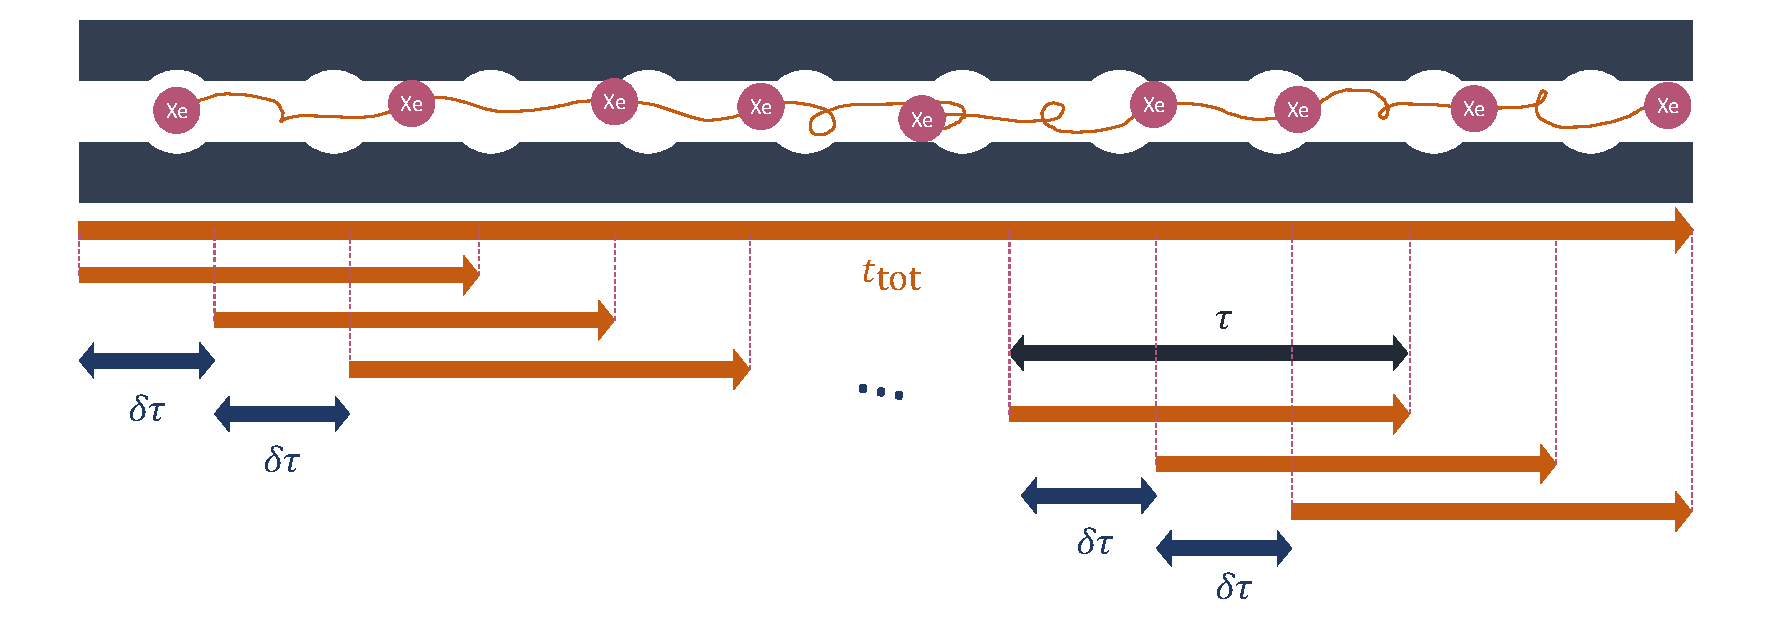
\includegraphics[width=0.95\textwidth]{figures/5-diffusion/diffusion_averaging.pdf}
    \caption{Illustration of the generation of trajectories of size $\tau$ by shifting the origins of multiple durations $\delta\tau$. }\label{fgr:window_msd}
\end{figure}

The major drawback of this method is that we need to define a timescale $\left\{\delta\tau, \ldots, K\delta\tau\right\}$ beforehand. In order to be able to access the different timescales in a single simulation, we can perform a multiple window algorithm developed by Dubbeldam et al.\ and used in the RASPA software to compute mean squared displacements (MSD) in a molecular dynamics simulation.

The different time windows are defined in a recursive way using the default parameters of RASPA. The first time window is defined by $K=25$ displacements of duration $\delta t, 2\delta t, \ldots,K\delta t$ with a shift of $\delta t$ (the default shift value $\delta t$ of the first window can be changed with the parameter SampleMSDEvery). The second window is now based on a sampling duration $\delta \tau_1 = K\delta t$ and the sub-trajectories will have durations of $\left(\tau_1^{(1)} = \delta\tau_1\right),\ldots,\left(\tau_1^{(k)} = K\delta\tau_1\right)$. If we repeat the process recursively until no window can be generated anymore, and the $i$\e{th} window would have a sampling duraction of $\delta \tau_i = K^i\delta t$ and sub-trajectories durations of $\left(\tau_i^{(1)} = \delta\tau_i\right),\ldots,\left(\tau_i^{(k)} = K\delta\tau_i\right)$. The time scale $\delta \tau_i = K^i\delta t$ we sample follows a geometrical progression and very different time scales can be accessed using this method in order to find the time scale corresponding to the diffusion regime (linear relation between the MSD and the duration of the sub-trajectories used in the averaging). For example on Figure~\ref{fgr:MSD_init}, we can see the different timescales and the exponent value $b$ of a fit to a function of type $x \mapsto ax^b$ for the different time windows --- values of $b$ near $1$ can be associated to a diffusion regime. The determination of the diffusion coefficient is now reduced to a simple fitting problem that will be explained in more details in the presentation of the diffusion coefficient screening in section~\ref{sct:md_screening}.

This methodology can then be used replicated to thousands of structures to characterize the diffusion properties of these materials. Several screenings have already been carried out in the literature as presented in the chapter 1 in the section dedicated to transport property screenings. We will now dive a little deeper in the prediction of these quantities using machine learning.

\subsubsection{ML modeling}

In a very recent study, Daglar et al.\ used an ML model to predict the diffusion coefficient of a 100 thousand hypothetical MOFs using the data for about 5000 CoRE MOF structures.\autocite{Daglar_2022} Along with very standard geometrical descriptors, they used chemical composition descriptors and the heat of adsorption as the input features of their machine learning model to predict the diffusion coefficients of \ce{H2}, \ce{CH4}, \ce{N2} and \ce{He} in the different MOF materials of CoRE MOF 2019 (training) and of hMOF (testing). The combination of kinetic data with thermodynamic data for the characterization of MOf materials is a very interesting approach. However, the major drawback of most of the approaches in the literature is the lack of structure--property relationship to understand the microscopic origins of the diffusion coefficient values.

Simarly to what we have done on the thermodynamic screening (chapter 2--4), in our approach to tranport property screening, we will also start by drawing structure--property relationships between the diffusion coefficient and the geometrical descriptors of the MOF structures. And in an attempt to have a deeper understanding of the diffusion process, we will try to evaluate the diffusion activation energy using energy grid-based methods described in the literature. All these techniques aim at better predicting the diffusion coefficients either in a direct calculation or in an ML surrogate model. To achieve that, we will start by introducing the kinetic Monte Carlo approach that is less accurate than the MD approach but is indeed much more efficient.

\subsection{Lattice kinetic Monte Carlo}

The lattice kinetic Monte Carlo method relies on a pre-defined lattice of stable points corresponding to adsorption sites. Each site connected to another if there is a diffusion path (narrow channel) that connects them. To calculate the probability of transition from one site to another, we need to define a transition state in the narraow channel which correspond to the highest energy point on the minimal energy diffusion path (the saddle point). The probability of transition would therefore be defined with regard to the energy barrier to overcome in order to cross the channel. Once the lattice defined, we only need to propagate an adsorbate from one site to another using the different transition probabilities, which gives a coarse-grained trajectory compared to the one obtained in a MD simulation, but is perfectly usable to compute the MSD and calculate a diffusion coefficient.

\todo{Illustration}

\subsubsection{Transition state theory}

The transition state theory is usually used in chemistry to explain the kinetics of a reaction. To do so it compares the energy of the reactants before reacting and the one of the transition state to calculate the rate of the reaction. And it defines a reaction kinetic rate that explains the kinetics of a reaction.

In our case, we want to study the transition from a pore to another one by transitioning through a channel. It is also possible to define a diffusion rate that connects the adsorption sites of the pores using Bennet-Chandler 
\todo{Bennet-Chandler approach}\autocite{BENNETT1977}

\todo{what is a transition state for diffusion?}

\subsubsection{Construction of the lattice}

\todo{Detect TS, and bassins.}

Fast kinetic Monte Carlo
tutrast\autocite{Mace_2019} autre étude avant aussi

\todo{Generation of trajectories + similar techniques than previously presented to find the MSD}


\section{Screening of transport properties}\label{sct:md_screening}

To complete the thermodynamic screenings that we performed in the chapters 2--4, we also carried out a transport property screening. In this section, we will provide a description of the screening approach as well as the analysis of the diffusion coefficients compared with typical geometrical descriptors.

\subsection{Diffusion in a selective material}

Before going into the details of the screening study, we will present the approach adopted for the diffusion coefficient calculation using MSD values, on one example, SBMOF-1\autocite{Banerjee_2016}. This preliminary study will help us calibrate the time parameters (time step, maximum time) that will be used in the final screening study.

First, I ran a molecular dynamics simulation of 500 million steps (about 1--2 days of simulation) with a thousand initialization steps and 100 thousand equilibration steps to model a xenon diffusing in the KAXQIL\autocite{Banerjee2012} MOF at infinite dilution. To be at infinite dilution, we set the box size so that no interactions occur between the different adsorbates. And we can observe on the Figure~\ref{fgr:MSD_init}, the different time scales at which different transport phenomena occur. 

From \SI{1}{\fs} to \SI{1}{\ps}, there is a ballistic regime with a squared dependence of the mean squared displacement. For a particle of mass $m$, the MSD $\langle {r(\tau)}^2 \rangle$ in this regime follows a simple ballistic relation (length equals velocity multiplied by time):
\begin{equation}
  \langle {r(\tau)}^2 \rangle = v_m^2 \tau^2 = \frac{k\e{B}T}{2\pi m}\tau^2
\end{equation}
where $v_m$ is the average velocity of a particle that follows the Maxwell-Boltzmann distribution at temperature $T$. If we calculate the squared mean velocity $v_m^2$ using the standard Maxwell-Boltzmann relation, we get a value of \SI{3}{\square\m\per\square\second}, which is very close to the value of \SI{2.8}{\square\m\per\square\second} obtained by the fit shown right plot of Figure~\ref{fgr:MSD_init}. This first regime simply corresponds to the movement of the particles subjected to the thermal agitation and is of little interest for diffusion. 

\begin{figure}[ht]
  \centering
    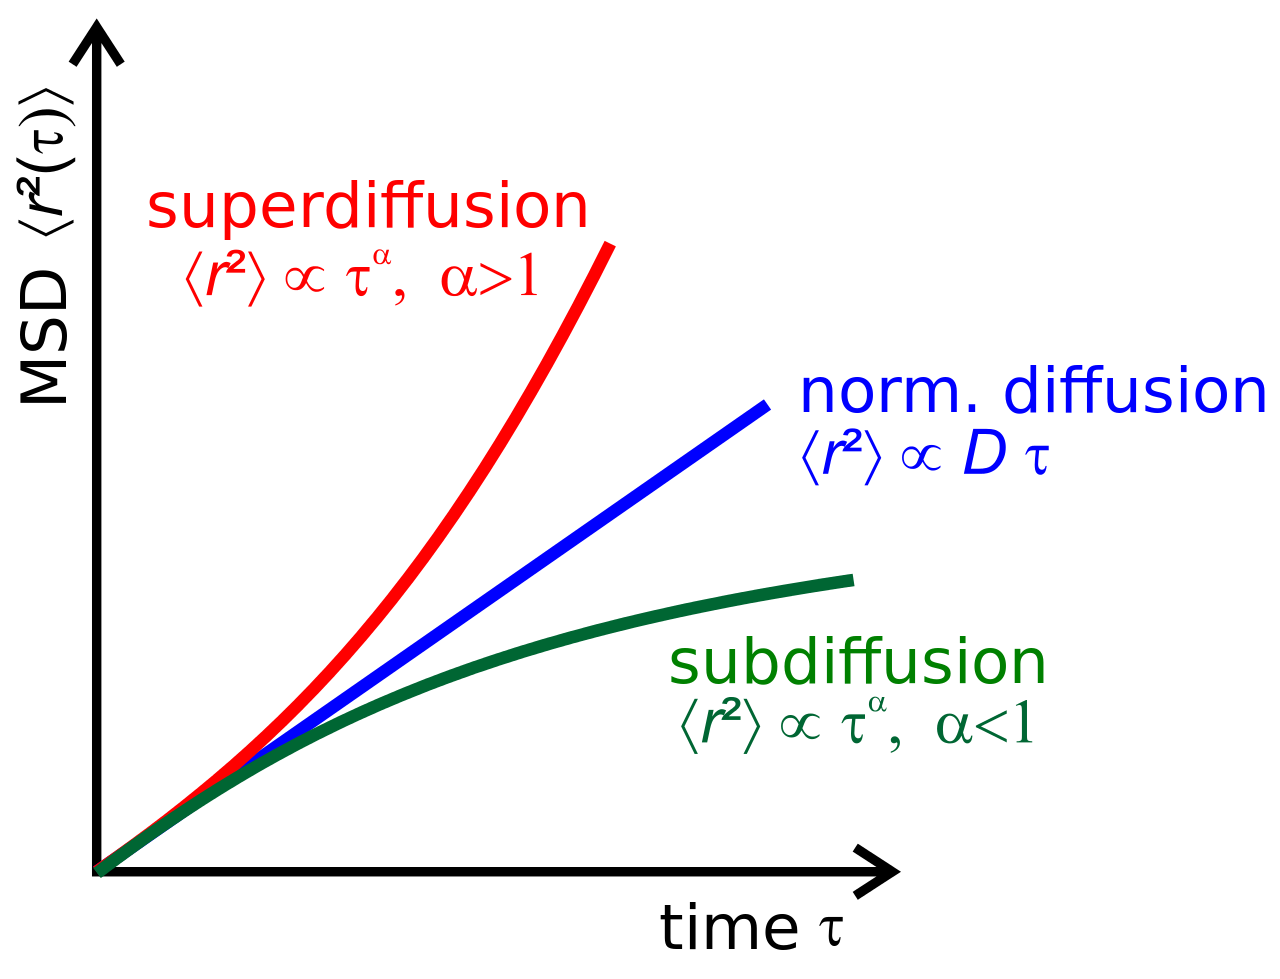
\includegraphics[width=0.48\textwidth]{figures/5-diffusion/Msd_anomalous_diffusion.svg.png}
    \includegraphics[width=0.48\textwidth]{figures/5-diffusion/MSD_Xe_KAXQIL_clean.pdf}
    \caption{Left: Different regimes that could be observed in an MSD plot as a function of time. The ballistic regime can be considered superdiffusional, the normal diffusion is simply a linear relation as described in the Einstein equation\ref{eq:einstein}, and the subdiffusion regime often occurs in obstructed media like nanoporous materials. \todo{redo} The different regimes can be found on the right plot of an actual MSD calculated using the multiple window method. The fittings are done using a generic function $K_\alpha\tau^\alpha$ and the exponents $\alpha$ are given in the legend. }\label{fgr:MSD_init}
\end{figure}

Then, there is a transition from the ballistic regime to the pseudo-diffusional regime (the exponent does not reach $1$ yet) that we observe in cyan on the plot. Between \SI{1}{\ps} and \SI{100}{\ps}, there is a so-called subdiffusion regime, where the MSD has a power function of the time $\langle {r(\tau)}^2 \rangle=K_\alpha\tau^\alpha$ with an exponent inferior to $1$ as illustrated on the left plot of Figure~\ref{fgr:MSD_init}. This regime corresponds to the confinement of the xenon particle inside an adsorption pore, there is only thermal vibration occuring and no diffusion hopping is observed at this time scale. And diffusion seems to start occuring at the \SI{10}{\ns} time-scale. As we can see on the Figure~\ref{fgr:MSD_linear_init}, the MSD between \SI{0.01}{\ns} and \SI{0.4}{\ns} really represents a sub-diffusional regime due to the confinement imposed by the nanopores of KAXQIL, but at \SI{0.4}{\ns}--\SI{9}{\ns}, the MSD start to have an exponent closer to $1$ and a linear fit is possible although not perfect. Ideally, we would want to sample trajectories in the order of tens of nanoseconds, which is the next time-scale. But with an MD time step of \SI{1}{\fs}, this would mean multiplying the computation time by at least 5 (1--2 weeks for one MD simulation), which begins to be prohibitive. 

\begin{figure}[ht]
  \centering
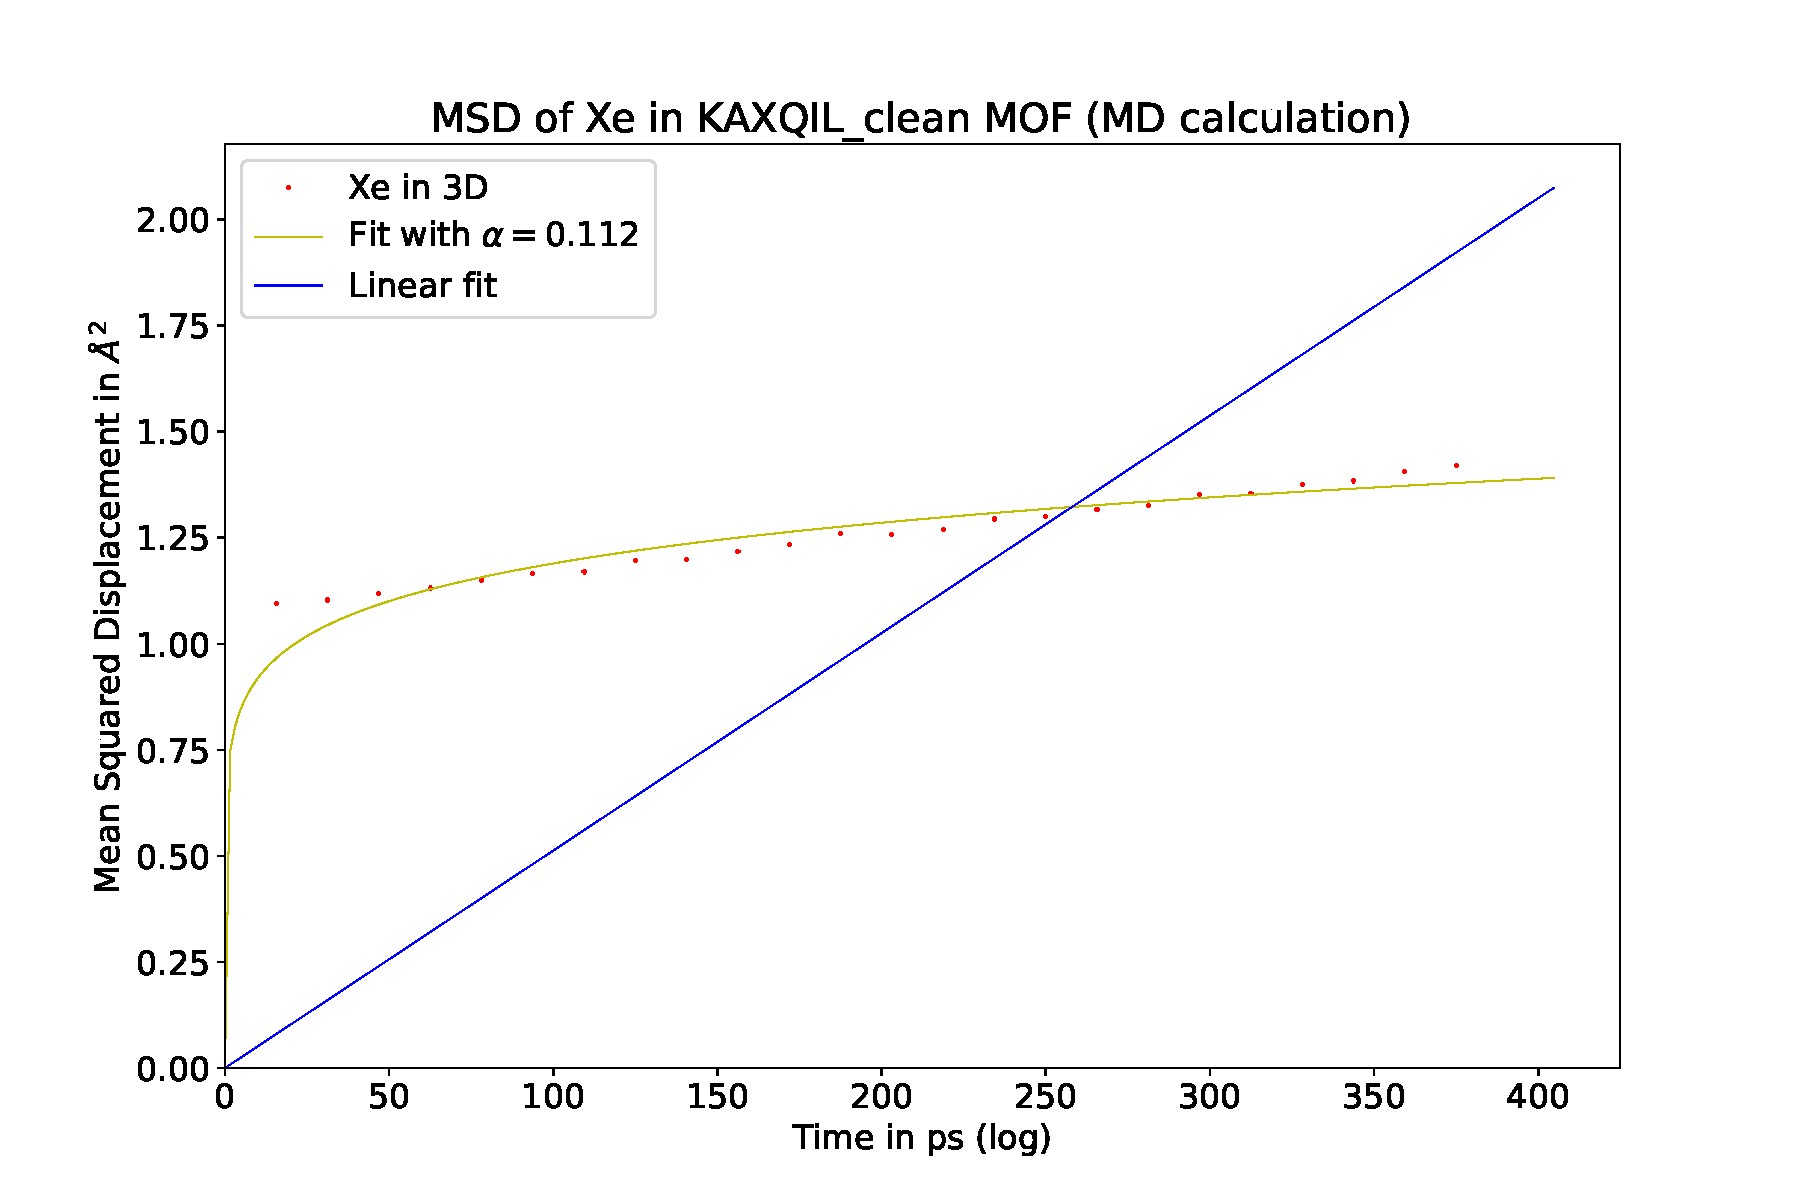
\includegraphics[width=0.48\textwidth]{figures/5-diffusion/MSD_Xe_coeff_KAXQIL_clean_1.pdf}
\includegraphics[width=0.48\textwidth]{figures/5-diffusion/MSD_Xe_coeff_KAXQIL_clean_2.pdf}
\caption{ Plots of the MSD at the last two time scales considered on the Figure~\ref{fgr:MSD_init}. On the left, the time-scale between \SI{0.01}{\ns} and \SI{0.4}{\ns} is considered, the MSD is fitted by a power function with the same exponent as one determined earlier, and a linear fit is given to show the incompatibility with the diffusion equation. On the right, we have the same approach but for the time-scale between \SI{0.4}{\ns} and \SI{9}{\ns}. }\label{fgr:MSD_linear_init}
\end{figure}

If we use the right plot of Figure~\ref{fgr:MSD_linear_init} to fit a linear relation and deduct the diffusion coefficient, we can have an underestimated value of the diffusion coefficient of $2.24\times 10^{-8}$~\si{\square\cm\per\square\s} --- it is an underestimation because the MSD is rather concave, which reduces the slope in the fitting process. This value is already a good estimation of the diffusion coefficient considering the rather high exponent $\alpha$ value in the with regard to $K_\alpha\tau^\alpha$.

Since there is an element of randomness in the initial position of xenon (pockets have been blocked so that xenon is not blocked), we need to measure the effet of running different MD simulations of the value of the diffusion coefficients. To measure this uncertainty across different MD simulations with different initial positions determined by with different random seed. In RASPA, the random seed is simply equal to the UNIX time upon launching the MD simulation. This ensures that a different random seed is given to the $10$ different MD simulations we launched using the exact same parameters as mentioned previously. We found that the average diffusion coefficient value equals $2.13\times 10^{-8}$~\si{\square\cm\per\square\s} and the standard deviation equals $0.37\times 10^{-8}$~\si{\square\cm\per\square\s}, which represents about {17\%} of the average value. We could estimate the uncertainty to about {17\%} on the diffusion coefficient for a rather low coefficient around $10^{-8}$~\si{\square\cm\per\square\s}, we could expect lower uncertainty for less obstructing materials. 

Now that we have more confidence on the method we are using, we will try to probe higher time-scales than the one accessible with an MD time step of \SI{1}{\fs}, because the diffusion regime seems to be occuring rather at the \SI{10}{\ns} time-scale. We ran a first calculation with 500 million step to confirm that we obtain a similar diffusion coefficient value. The time window between \SI{2}{\ns} and \SI{47}{\ns}, and the MSD are calculated from about 200 sampled trajectories, which gives rather correct values. We can obtain a more accurate diffusion coefficient of $2.6\times 10^{-8}$~\si{\square\cm\per\square\s}, which is very close to the one obtained in the previous approach. The value is slightly higher (which is expected) since the previous values was over-estimated. This approach is therefore consistent with the previous one.

To further back-up the use of a higher time integration step, we need to understand the origin of the value of \SI{1}{\fs}. This value is usually justified by the Nyquist-Shannon sampling theorem that implies the integration step to be at most half of the period of the fastest vibration within the system. If we take a C--H vibration, the maximum time step value is \SI{5}{\fs}, and to be on the safe side, a time step of $1$--$2$~\si{\fs} is chosen in most of the diffusion studies in nanoporous materials.\autocite{Bukowski_2021} But in our system of a xenon diffusing in a rigid environment, we actually don't have any vibrational limitations as described earlier. I think that the use of higher time steps in this situation can be an easy way to access higher time-scales; however, furhter studies need to be performed to be sure of the validity of the quantities we derive from these MD simulations. The value of \SI{5}{\fs} is on the higher side of what we usually see in MD simulations, but it can be justified by the rigidity of the framework and the adsorbate we consider. Even higher time steps could be tested, but to be sure of the results we stay at this reasonable middle ground of \SI{5}{\fs} for all our high-throughput screening of the transport properties.

\todo{talk about superdiffusion for KAXQIL. Maybe landauer blowtorch effect.}
When probing the much higher time-scale of 50--950~\si{\ns}, I came across an anomalous diffusion regime that corresponds to a surdiffusion according to the plot...



\subsection{Structure--diffusivity relationships}


500 000 000 cycles with restart on the server. order of 2--3 days per structures
Requires 2 to 3 restarts. Still some structures did not finish within this time frame but the incomplete MSD can however be anlyzed.

\todo{We have generated diffusion coefficients for the ... best materials}

\todo{correlation with VF/SA/Selectivity/permselectivity}

\begin{figure}[ht]
  \centering
    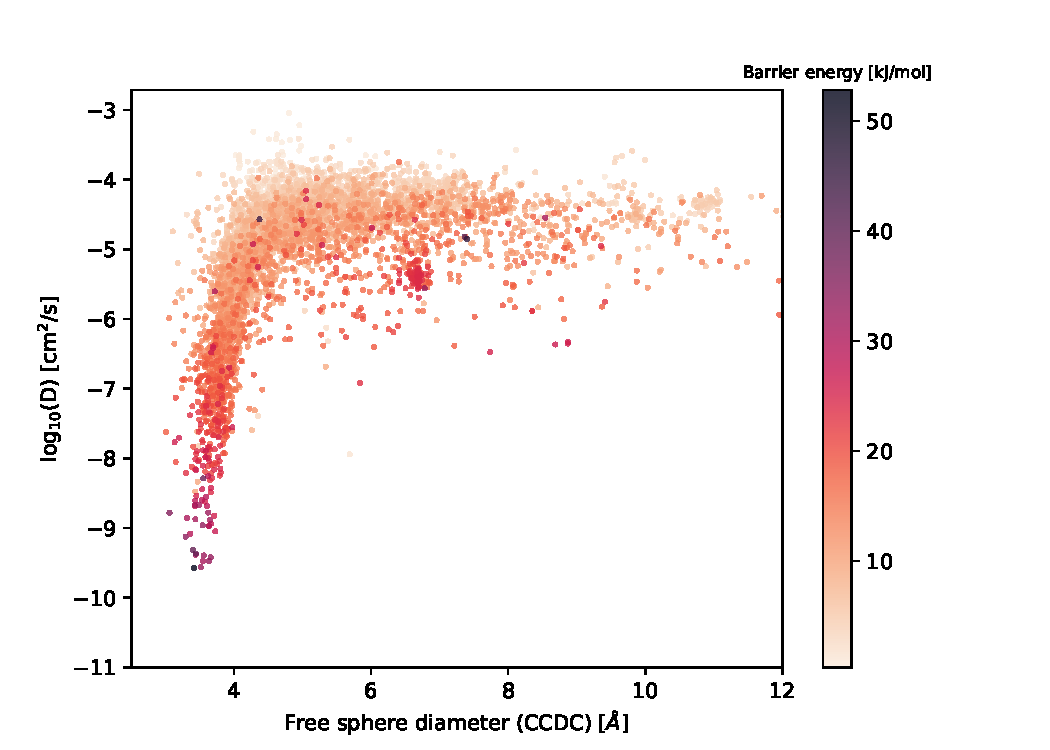
\includegraphics[width=0.48\textwidth]{figures/5-diffusion/difflog_Df-ccdc_barrier.pdf}
    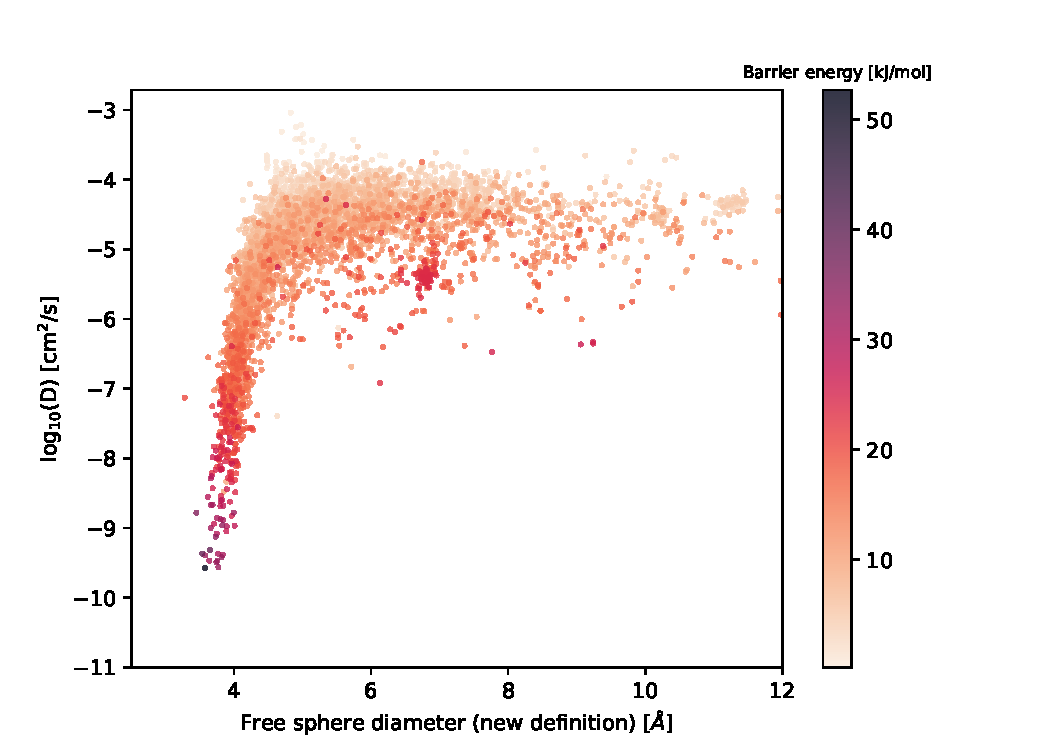
\includegraphics[width=0.48\textwidth]{figures/5-diffusion/difflog_Df-uff298K_barrier.pdf}
    \caption{\todo{correlation with PLD without labeling}}\label{fgr:}
\end{figure}


% Outre l'exemple très parlant de SBMOF-1, d'autres publications, dans la séparation d'hydrocarbures notamment, s'intéressent aux éventuelles blocages cinétiques grâce à des simulations de dynamique moléculaire (MD) flexible.\cite{Stanton_2022} Ils ont notamment mis en évidence que la diffusion pouvait détériorer les performances de structure présentant d'excellente performance thermodynamique (énergie d'adsorption). Cette approche est très complète, car elle allie la thermodynamique, la flexibilité et les effets de transport dans une seule étude. En revanche, elle est très coûteuse en temps de calcul et ne pourrait être appliquée qu'à une poignée de structures. Au lieu d'utiliser des champs de force flexible qui alourdissent énormément la simulation, il est possible de se tourner vers une approche en ``snapshot'' bien moins coûteuse que nous développerons dans la dernière partie de ce rapport. Dans cette partie, nous nous focaliserons uniquement sur le couplage thermodynamique/cinétique.

% Afin de recouper nos données purement structurelles et thermodynamiques avec des propriétés de transport, on a effectué un screening des coefficients de diffusion du xénon et du krypton sur les 7822 structures les plus sélectives. 
% Des trajectoires de dynamique moléculaire ont été calculées sur l'ensemble de ces structures deux fois pour chaque adsorbat à dilution infinie. Il a fallu environ une à deux journées de simulation par structure afin de déterminer leurs coefficients de diffusion. Il est à noter pour la suite que les valeurs de diffusivités sont déterminés à l'ordre de grandeur près. Autrement dit c'est l'échelle logarithmique qui est pertinent pour les comparer à d'autres grandeurs. On a pu établir une forte corrélation entre le coefficient de diffusion et la taille minimale des canaux de diffusion à l'intérieur du matériau (PLD). La figure~\ref{fgr:Diff_Df_s} met en évidence la corrélation linéaire entre le logarithme de la diffusivité et le LCD pour des canaux de taille inférieure au diamètre cinétique du xénon (\SI{4,3}{\angstrom}). Ensuite, on arrive sur un plateau, c'est-à-dire que la diffusion du xénon dans le matériau ou dans le vide sont quasiment équivalentes. Les canaux sont assez larges pour permettre la libre diffusion du xénon à l'intérieur de ces matériaux. On voit aussi que ces matériaux ont moins de chances d'être sélectifs (les points foncés sont plus rares). Cette corrélation ouvre la voie au développement de modèles statistiques pour prédire la diffusivité, ce qui a déjà été étudié par Daglar \emph{et al.} dans leur récente publication.\cite{Daglar_2022} Dans leur étude, pour l'hélium, le coefficient de corrélation entre les coefficients de diffusion prédites et calculés par MD est d'environ 0,65 pour les données de test, ce qui n'est pas très précis. Il faut donc nuancer l'approche ``machine learning'' pour la prédiction des diffusivités. Cependant, l'étude n'a pas encore été menée sur le xénon et le krypton, ce qui pourrait mériter une étude préliminaire.

\begin{figure*}[t]
\centering
  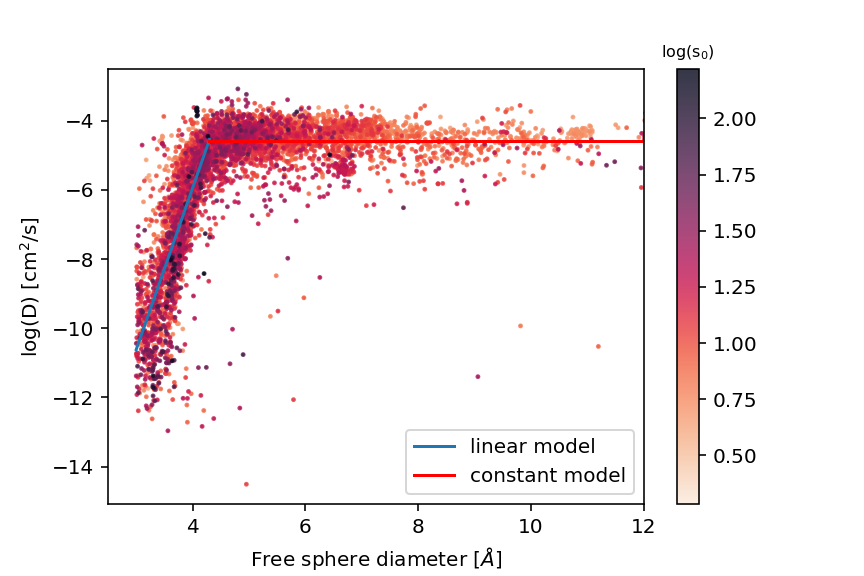
\includegraphics[width=0.8\textwidth]{figures/5-diffusion/D_log-diameter_colored_s_models+.png}
  \caption{Logarithme du coefficient de diffusion du xénon à la limite des basses pressions en fonction du diamètre de la plus petite sphère libre dans le matériau (LCD). Les points sont colorés en fonction du logarithme de la sélectivité à basse pression $\log(s_0)$.}\label{fgr:Diff_Df_s}
\end{figure*}


\subsection{Identification of interesting materials}


% En analysant les rapports des coefficients de diffusion en comparaison des sélectivités, on a pu identifier deux structures qui couplent une bonne sélectivité à un ratio de diffusivités autour de 0,5 (\emph{cf.} table~\ref{table:diff}) : les structures de code CCSD GUMDEZ et QOZDOY. Grâce à leur LCD proches du diamètre cinétique du xénon et à un PLD assez élevé pour ne pas entraver le déplacement du xénon à travers les canaux. Les coefficients de diffusion du xénon tournent autour de 7$\times$10\ex{-5} \SI{}{\square\centi\meter\per\second} ce qui est proche de la diffusion libre (de l'ordre de 10\ex{-5} \SI{}{\square\centi\meter\per\second}), ce qui confirme l'absence de blocage cinétique. 

% Une autre structure, ADOGEH (\emph{cf.} table~\ref{table:diff}), présente une diffusion 14 fois plus rapide pour le xénon que le krypton, tout en ayant une sélectivité à basse pression de 49. Ce phénomène s'explique par le fait que la structure a des canaux dans les trois directions et que pour changer de direction il faut passer par un canal plus étroit non accessible par le xénon. Ainsi le xénon, n'ayant qu'une direction de diffusion à l'intérieur du matériau, va bien plus vite que le krypton pour lequel toutes les directions s'offrent à lui. Ainsi, le krypton est plus lent à diffuser car il change de direction constamment dans le matériau contrairement au xénon. En revanche, la sélectivité baisse à 10 lorsque l'on considère un mélange de 20/80 Xe/Kr à pression ambiante au lieu de la dilution infinie. Ce matériau pourrait être utile notamment à pression partielle faible en xénon et krypton, ce qui est le cas pour notre application. Des études plus approfondies sont encore à mener, notamment en confirmant les valeurs de sélectivité par des calculs DFT plus fiable ou en étudiant la flexibilité ; mais si les résultats sont concluant ces matériaux pourraient alors être testés expérimentalement pour une éventuelle application industrielle.

\begin{table}[ht]
\centering
\begin{tabular}{|l|r|r|r|r|r|r|}
\hline
  CCSD ref.\ code &      LCD (\SI{}{\angstrom}) &    s$_1$ &       s$_0$ &     PLD (\SI{}{\angstrom}) &     Ratio Diff. &  Coeff.\ de Diff. Xe \\
\hline
QOZDOY\cite{Zhang_2001} &  5,3 & 37 & 52 & 4,7 &  0.4 &               7$\times$10\ex{-5} \SI{}{\square\centi\meter\per\second} \\
GUMDEZ\cite{Yin_2014} &  5,3 & 42 & 56 & 4,8 &  0.5 &               7$\times$10\ex{-5} \SI{}{\square\centi\meter\per\second} \\
ADOGEH\cite{Peikert_2012} & 12,7 &  10 & 49 & 5,1 & 14 &               5$\times$10\ex{-5} \SI{}{\square\centi\meter\per\second} \\
\hline
\end{tabular}
\caption{Performances de structures identifiées par un screening prenant en compte les coefficients de diffusion. }\label{table:diff}
\end{table}

% Les résultats d'un screening couplant thermodynamique et cinétique permettent déjà de mettre en valeur des matériaux encore inconnus de la communauté. La question du blocage cinétique est certes traitée dans certaines études,\cite{Stanton_2022} mais aucune approche systématique n'a encore été développée. Ces structures ont des sélectivités élevées mais ne sont pas les plus sélectives; elles auraient donc été écartées dans un screening standard basé uniquement sur la thermodynamique. 

% Cette approche basée sur des trajectoires de dynamique moléculaire présente toutefois ses propres défauts. En effet, la méthode est très lente (quelques jours de simulation par structure), les structures avec différents canaux non connectées posent problème car l'adsorbat ne peut diffuser que dans un seul des deux canaux. Ainsi, il faudrait dans certains cas faire plusieurs trajectoires ce qui demande encore davantage de temps de calcul. De plus, si l'on veut ajouter de la flexibilité, cette méthode ne pourrait être utilisée que sur quelques structures. C'est pourquoi, un algorithme bien plus efficace est en cours d'implémentation en C++ pour accélérer les calculs de diffusivité. Un tel algorithme est déjà conçu par le groupe de Berend Smit à l'EPFL \cite{Mace_2019}, mais le code étant sous Matlab (langage peut efficace), il est impossible de l'utiliser dans des procédures de screening. Cet algorithme détermine des sites d'adsorption et des états de transition pour passer d'un site à un autre. Puis à l'aide de simulations de Monte Carlo cinétique l'adsorbat se déplace d'un site à un autre au rythme d'une constante cinétique déterminée par l'état de transition. Cette méthode permet également d'identifier en avance les différents canaux et on assure que chacun d'entre eux sont traversés par des molécules. Par conséquent, ce nouveau code permettrait de résoudre les problèmes de temps de calcul et de fiabilité rencontrés avec la dynamique moléculaire. 

\section{Fast diffusion calculation algorithm}

\subsection{Implementation in C++}

Breadth-first search

\subsection{Preliminary results}

\subsection{Visualization tool}

\todo{Take some examples for the vizualisation with comparison to the pore size and diffusion coefficient}

\subsection{Development of a first prediction model}

\begin{figure}[ht]
  \centering
    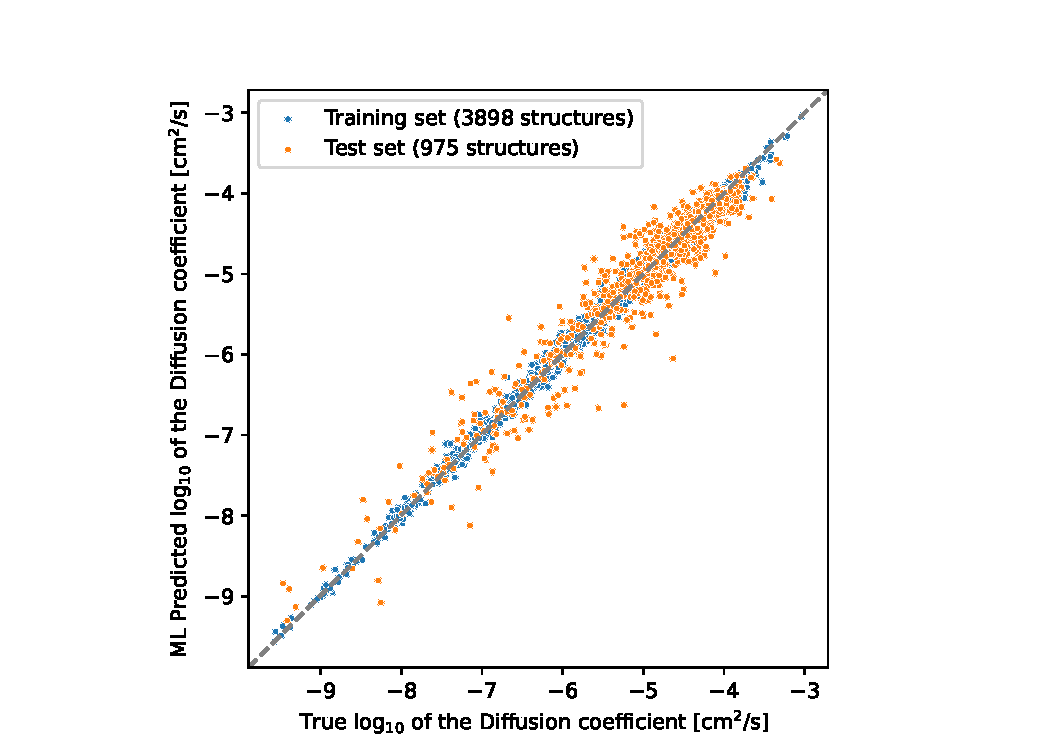
\includegraphics[width=0.48\textwidth]{figures/5-diffusion/diffusion_prediction.pdf}
    \caption{}\label{fgr:}
\end{figure}

\begin{figure}[ht]
  \centering
    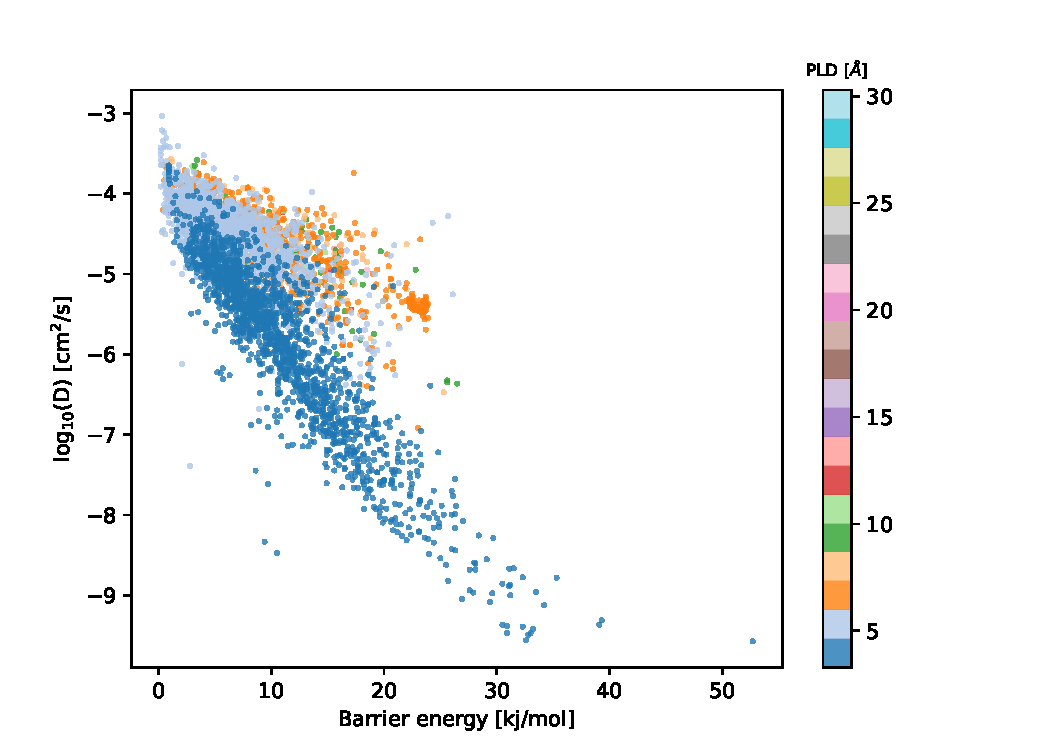
\includegraphics[width=0.48\textwidth]{figures/5-diffusion/difflog_barrier_Df_uff.pdf}
    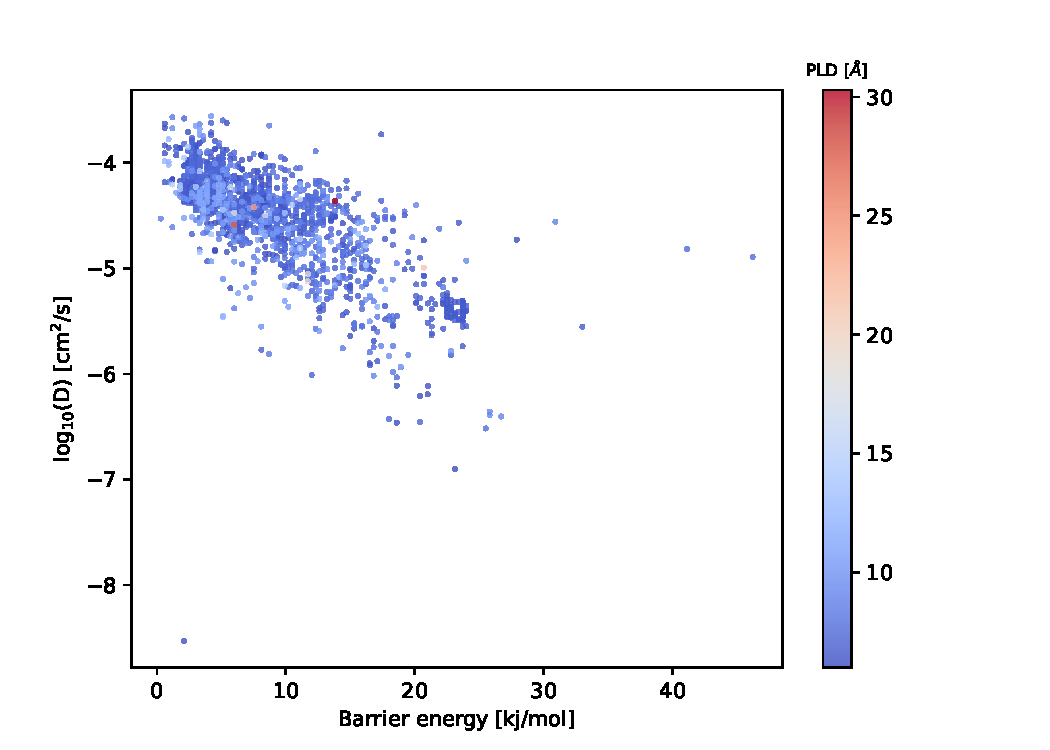
\includegraphics[width=0.48\textwidth]{figures/5-diffusion/difflog_barrier_Df_uff_2.pdf}
    \caption{}\label{fgr:}
\end{figure}

\begin{figure}[ht]
  \centering
    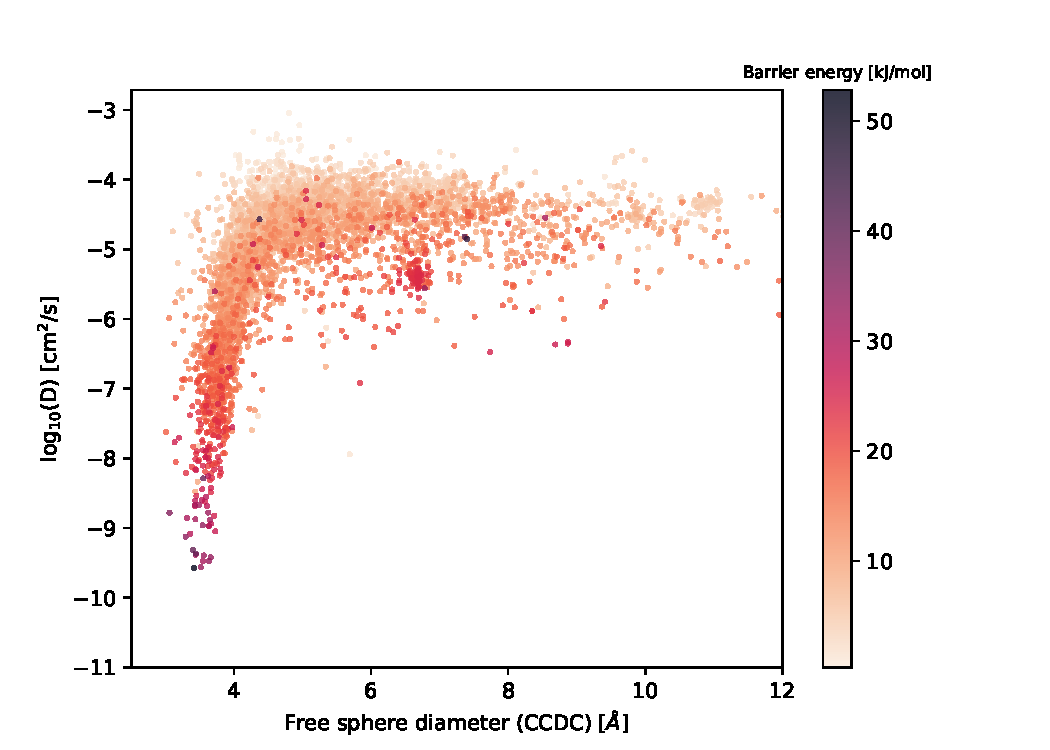
\includegraphics[width=0.48\textwidth]{figures/5-diffusion/difflog_Df-ccdc_barrier.pdf}
    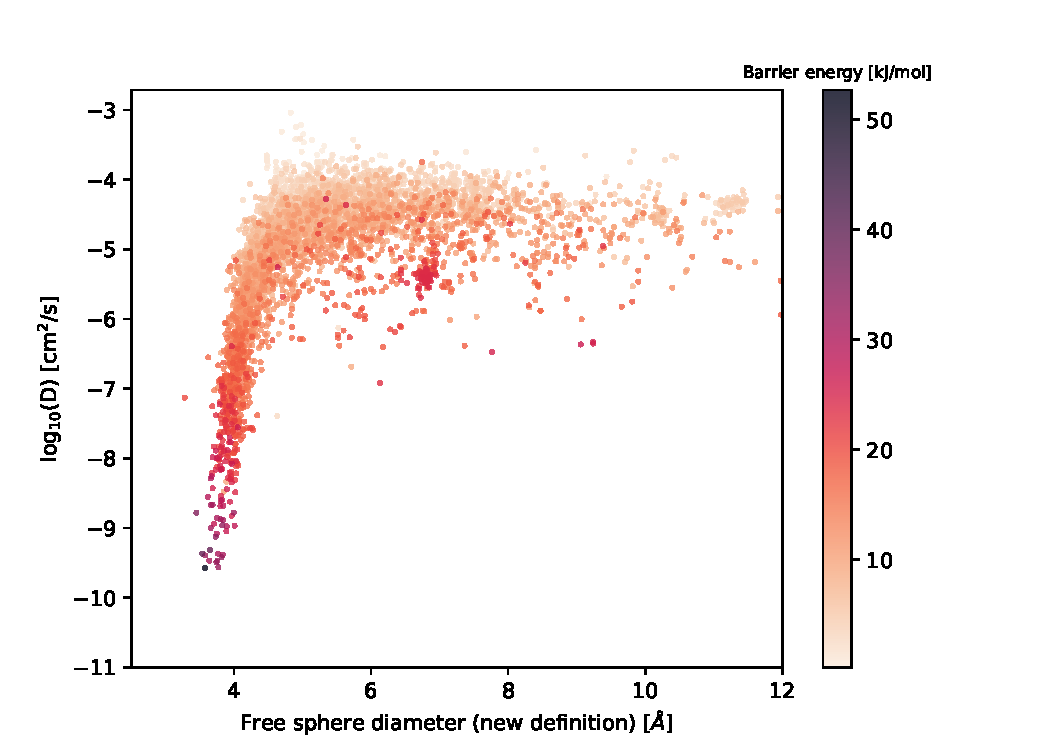
\includegraphics[width=0.48\textwidth]{figures/5-diffusion/difflog_Df-uff298K_barrier.pdf}
    \caption{}\label{fgr:}
\end{figure}

ML descriptors

\textbf{Next steps}

\todo{Broaden to the study of collective diffusion, Maxwell-stefan, Onsager, etc.}

\todo{Can be used in breakthrough simulations using RUPTURA and equations that link the diffusion coefficient to the axial dispersion coefficient a key parameter in the breakthrough modeling.}\autocite{Sharma_2023}

\OnlyInSubfile{\printglobalbibliography}

\end{document}
